\documentclass[tikz,border=5]{standalone}
\usepackage[utf8]{inputenc}
\usepackage[T1]{fontenc}
\usepackage{amsmath}
\usepackage{amssymb}
\usepackage{tikz}
\usetikzlibrary{shapes,arrows}

\begin{document}

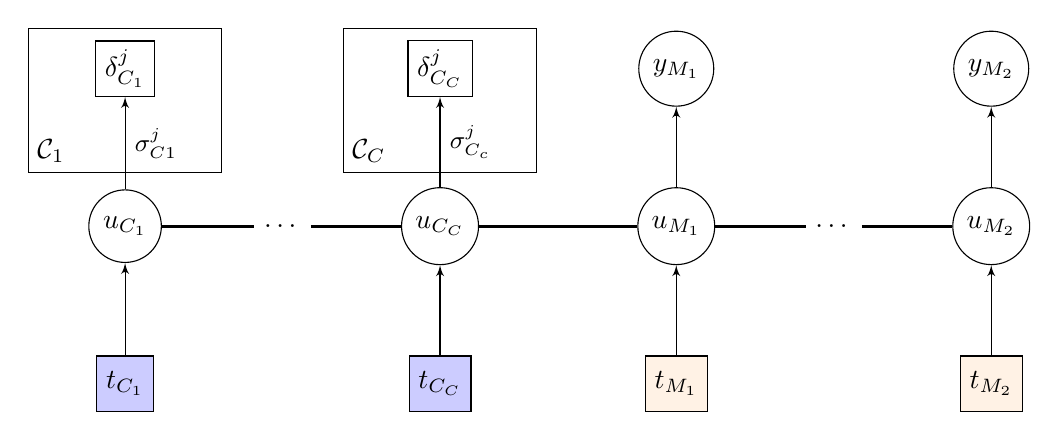
\begin{tikzpicture}
		\tikzset{vertex/.style = {shape=circle,draw,minimum size=1.5em}}
		\tikzset{vertex_obs/.style = {shape=rectangle,draw,minimum size=2em}}
		\tikzset{vertex_text/.style = {draw=white!80,minimum size=2em}}
		\tikzset{group/.style = {shape=rectangle,draw,minimum height=5.2em, minimum width=7em}}
		\tikzset{edge/.style = {->,> = latex'}}
		% vertices
		% --- Corr1
		\node[vertex_obs,fill=blue!20] (x1) at  (0,0) {$t_{C_1}$};
		\node[vertex] (f1) at  (0,2) {$u_{C_1}$};
		\node[vertex_obs] (y1) at  (0,4) {$\delta_{C_1}^j$};
		\node[group,text height=0.5em] (y1group) at  (0,3.6) {};
		\node[above right,text height=0.5em] at (y1group.south west) {$\mathcal{C}_1$};
		% --- div
		\node[vertex_text] (fdots) at  (2,2) {$\dots$};
		% --- Corr2
		\node[vertex_obs,fill=blue!20] (x2) at  (4,0) {$t_{C_C}$};
		\node[vertex] (f2) at  (4,2) {$u_{C_C}$};
		\node[vertex_obs] (y2) at  (4,4) {$\delta_{C_C}^j$};
		\node[group,text height=0.5em] (y2group) at  (4,3.6) {};
		\node[above right,text height=0.5em] at (y2group.south west) {$\mathcal{C}_C$};
		% --- Corr1
		\node[vertex_obs,fill=orange!10] (xM1) at  (7,0) {$t_{M_1}$};
		\node[vertex] (fM1) at  (7,2) {$u_{M_1}$};
		\node[vertex] (yM1) at  (7,4) {$y_{M_1}$};
		\node[vertex_obs,fill=orange!10] (xM2) at  (11,0) {$t_{M_2}$};
		\node[vertex] (fM2) at  (11,2) {$u_{M_2}$};
		\node[vertex] (yM2) at  (11,4) {$y_{M_2}$};
		\node[vertex_text] (fdots2) at  (9,2) {$\dots$};
		%edges
		\draw[edge] (x1) to node [font=\small,left]{} (f1);
		\draw[edge] (f1) to node [font=\small,right]{$\sigma_{C1}^j$} (y1);
		\draw[edge] (x2) to node [font=\small,left]{} (f2);
		\draw[edge] (f2) to node [font=\small,right]{$\sigma_{C_c}^j$} (y2);
		\draw[edge] (xM1) to node [font=\small,left]{} (fM1);
		\draw[edge] (fM1) to node [font=\small,left]{} (yM1);
		\draw[edge] (xM2) to node [font=\small,left]{} (fM2);
		\draw[edge] (fM2) to node [font=\small,left]{} (yM2);
		\draw[very thick] (f1) edge[-] (fdots);
		\draw[very thick] (fdots) edge[-] (f2);
		\draw[very thick] (f2) edge[-] (fM1);
		\draw[very thick] (fM1) edge[-] (fdots2);
		\draw[very thick] (fdots2) edge[-] (fM2);
	\end{tikzpicture}

\end{document}